\section{Hallazgos de Tesis}

\begin{frame}{Fuerza Capilar ($FC$): Identificación de Macro-Hubs}
  \begin{columns}[T]
    \begin{column}{0.55\textwidth}
      \begin{itemize}
        \item \textbf{Fuerza Capilar ($FC_H$):} Cuantifica la convergencia de flujos y la capacidad de un nodo 
                para actuar como transferencia intermodal.
        \item \textbf{Macro-Hubs:} Agrupaciones de estaciones (radio 100m) que consolidan el transbordo físico 
                (ej. CETRAMs).
        \item \textbf{Nodos Críticos Detectados:} 
        \begin{itemize}
            \item \textit{Chimalcoyotl-Coapa}: $FC_H = 134$.
            \item \textit{Acoxpa-Tlalpan}: $FC_H = 117$.
            \item \textit{Alpes-Periférico Sur}: $FC_H = 92$.
        \end{itemize}
      \end{itemize}
    \end{column}
    \begin{column}{0.40\textwidth}
      \begin{figure}
        \centering
        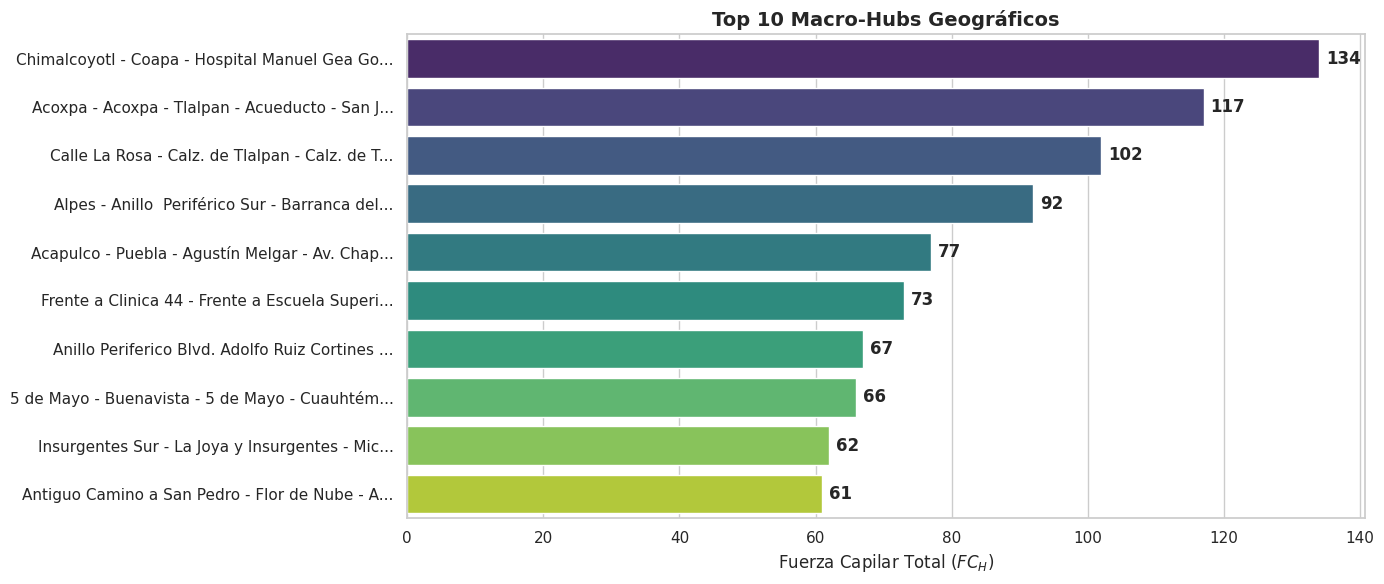
\includegraphics[width=\textwidth]{img/Top10Macrohubs.png}
        \caption{\tiny Top 10 Macro-Hubs Geográficos \cite{garibaldi2023vft}.}
      \end{figure}
    \end{column}
  \end{columns}
\end{frame}

\begin{frame}{Fuerza Capilar ($FC$): Mapa de Macro-Hubs}
  \begin{columns}[T]
    \begin{column}{0.55\textwidth}
      \begin{itemize}
        \item \textbf{Dispersión de Nodos:} Aunque en teoría, la \zmvm solo tiene nodos específicos identificados como CBD y centros educativos, 
        el mapa revela que hay una serie de puntos importantes con una tendencia hacia el poniente, centro, norte y sur.
        \item \textbf{Nodos no reconocidos:} Varios de estos nodos no son CETRAMs reconocidos por la Secretaría de Movilidad, lo que representa 
        una falta de planeación  del transporte público y una vulnerabilidad en términos sociales por la alta aglomeración de gente.
        \end{itemize}
    \end{column}
    \begin{column}{0.40\textwidth}
      \begin{figure}
        \centering
        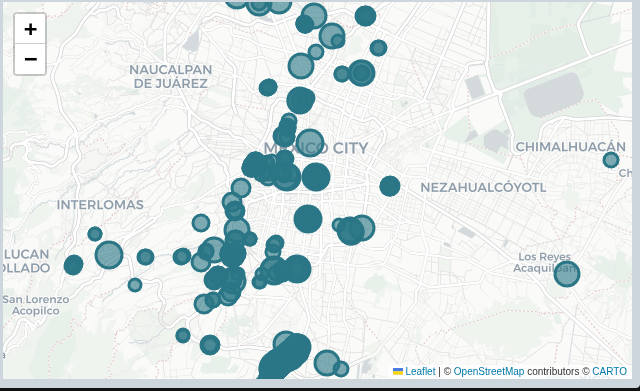
\includegraphics[width=\textwidth]{img/MacroHubsGeográficos.png}
        \caption{\tiny Top 10 Macro-Hubs Geográficos.}
      \end{figure}
    \end{column}
  \end{columns}
\end{frame}

\begin{frame}{Diagnóstico: Fragmentación y el Índice de Ruta Directa}
  \begin{itemize}
    \item \textbf{Mosaico de Retículas Desfasadas:} La periferia opera como parches aislados cuya trama interna no 
            se alinea con la red vial primaria.
    \item \textbf{Ineficiencia Geométrica ($DI$):} La desconexión obliga a trayectos radiales ineficientes, 
            elevando significativamente el \termino{Índice de Ruta Directa}.
    \item \textbf{Efecto Isla:} Los nodos periféricos actúan como destinos con conectividad lateral nula, forzando 
            viajes hacia el centro para conectar con zonas aledañas.
  \end{itemize}
  \begin{exampleblock}{Análisis de Red}
    Un usuario en el cuarto contorno puede enfrentar un $DI > 2.5$, lo que significa que recorre más del doble de la distancia 
        euclidiana necesaria .
  \end{exampleblock}
\end{frame}

% ========== DIAPOSITIVA 1: OPTIMIZACIÓN Y TABLA (IMAGEN) ==========
\begin{frame}{Recalibración Anillar: Optimización del Tiempo}
  \begin{columns}[c]
    % Columna Izquierda: Análisis
    \begin{column}{0.48\textwidth}
      \small
      \textbf{Reducción del Tiempo ($T$):}
      \begin{itemize}
        \item \scriptsize La simulación proyecta una reducción promedio de \textbf{20 minutos} por viaje en el sistema metropolitano.
        \item \scriptsize Eficiencia del modelo: $\Delta T \approx -24\%$.
      \end{itemize}
    \end{column}
    
    % Columna Derecha: Imagen de la Tabla de Eficiencia
    \begin{column}{0.48\textwidth}
      \begin{figure}
        \centering
        % Reemplaza "tabla_eficiencia.png" por el nombre real de tu archivo de imagen
        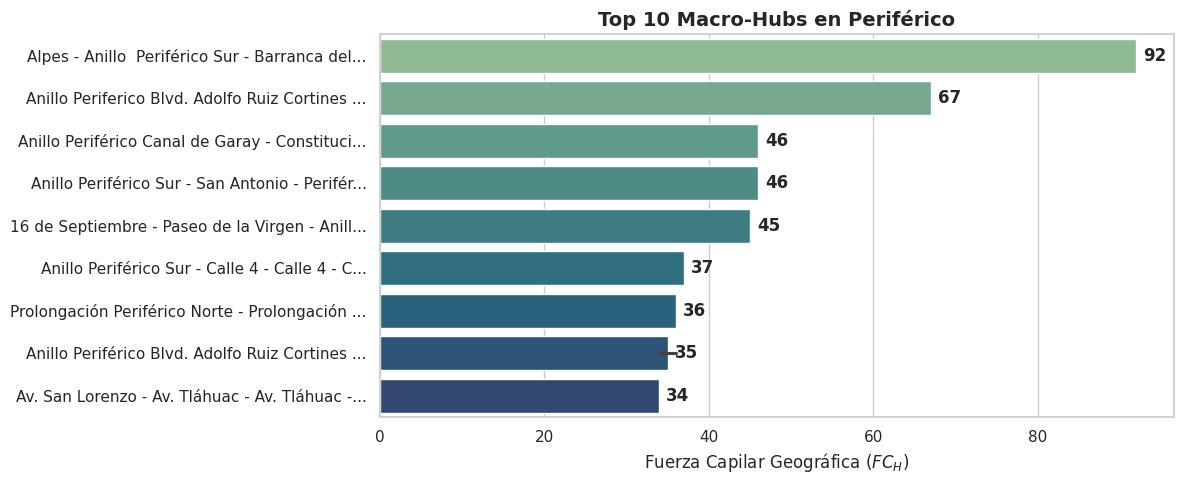
\includegraphics[width=\textwidth, height=0.65\textheight, keepaspectratio]{img/MAcroHubsPerifericoTabla.png}
        \caption{\tiny Proyección de Tiempos y Eficiencia ($\Delta T$).}
        \label{fig:opt_tiempo_imagen}
      \end{figure}
    \end{column}
  \end{columns}
\end{frame}



% ========== DIAPOSITIVA 2: ANCLAJES Y PRIMER MAPA ==========
\begin{frame}{Recalibración Anillar: Anclajes en Periférico}
  \begin{columns}[c]
    % Columna Izquierda: Análisis
    \begin{column}{0.48\textwidth}
      \small
      \textbf{Anclajes Naturales:}
      \begin{itemize}
        \item \scriptsize El eje \textit{Periférico Sur} concentra nodos con alta Fuerza Nodal ($FC$).
        \item \scriptsize \textit{Periférico-Tepalcates} registra un $FC_i = 20$.
        \item \scriptsize Funcionan como estaciones naturales de transferencia de infraestructura preexistente.
      \end{itemize}
    \end{column}
    
    % Columna Derecha: Mapa de Fuerza Nodal
    \begin{column}{0.48\textwidth}
      \begin{figure}
        \centering
        % Reemplaza con tu archivo de mapa correspondiente
        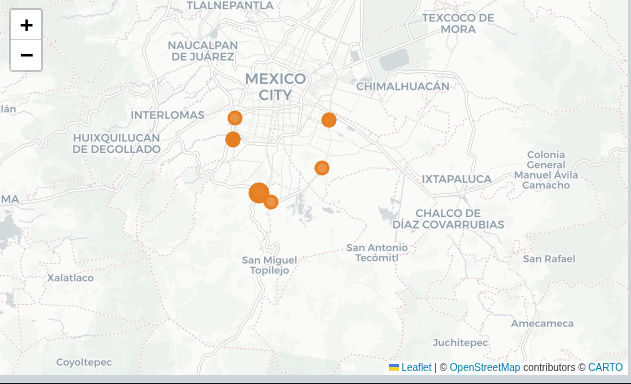
\includegraphics[width=\textwidth, height=0.65\textheight, keepaspectratio]{img/MacroHubsPerifericoMapa.png}
        \caption{\tiny Mapa 1: Distribución de Fuerza Nodal ($FC_i$).}
      \end{figure}
    \end{column}
  \end{columns}
\end{frame}


% ========== DIAPOSITIVA 3: CENTRALIDAD Y SEGUNDO MAPA ==========
\begin{frame}{Recalibración Anillar: Redistribución de Centralidad}
  \begin{columns}[c]
    % Columna Izquierda: Análisis
    \begin{column}{0.48\textwidth}
      \small
      \textbf{Estructura de Flujos:}
      \begin{itemize}
        \item \scriptsize El anillo mitiga la carga de intermediación ($B(v)$) en el núcleo histórico.
        \item \scriptsize Descompresión en \textit{Pino Suárez} y \textit{Tacubaya} en un \textbf{45\%}.
      \end{itemize}
      
      \vspace{0.2cm}
      
      \begin{block}{\tiny Nota Aclaratoria}
        \tiny El análisis de $FC$ identifica los puntos de anclaje ideales sin requerir aún un trazado geométrico final.
      \end{block}
    \end{column}
    
    % Columna Derecha: Mapa de Intermediación
    \begin{column}{0.48\textwidth}
      \begin{figure}
        \centering
        % Reemplaza con tu archivo de mapa correspondiente
        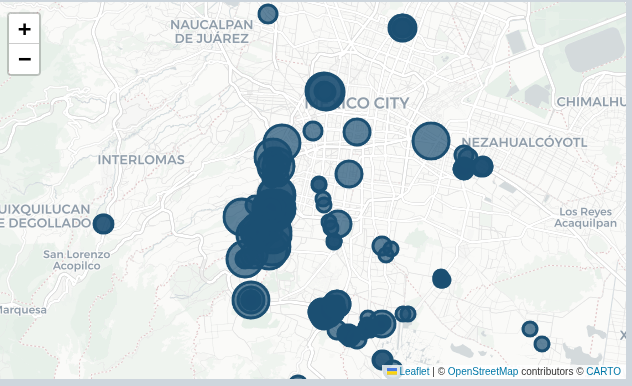
\includegraphics[width=\textwidth, height=0.65\textheight, keepaspectratio]{img/MacroHubsPerifericoMapa2.png}
        \caption{\tiny Mapa 2: Alivio de carga por intermediación ($B(v)$).}
      \end{figure}
    \end{column}
  \end{columns}
\end{frame}
